\section{Analisi \gloss{usabilità} di \fiscoloWeb}\label{usabilita-fiscolo}

Nella prima fase di stage mi è stato chiesto di studiare \fiscoloWeb{} per
familiarizzarmi con l'applicazione e capirne il funzionamento. Mi è stato
inoltre chiesto di segnalare eventuali problemi di usabilità, seguono gli esiti
di tale studio.

\subsection{Problematiche individuate}
Il sito non presenta grossi problemi di usabilità, ci sono però alcuni dettagli che,
se sistemati, potrebbero portare a un maggiore gradimento da parte degli/delle utenti.

\begin{itemize}
\item \textbf{Link e aree cliccabili}: è molto frustrante per un utente "sbagliare"
il click di un link, le aree cliccabili dovrebbero essere ben definite e non ambigue.
	\begin{itemize}
	\item La pagina di \textit{Scrivania} di \fiscoloWeb{} offre la possibilità di accedere
	alle funzionalità dei due sottomoduli \fiscolo{} e \resa{} attraverso due link
	composti da un logo e una \textit{tagline}, tra queste due parti è presente una piccola
	area non cliccabile che aumenta il rischio per un/a utente di "sbagliare" il click.
	Inoltre l'area cliccabile relativa alla tagline si estende fino a centro pagina senza
	offrire però indizi visibili.
	
	\begin{figure}[H]\label{imgDashboardLink}
		\centering
		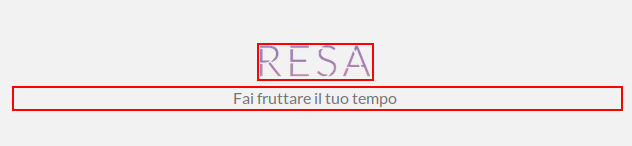
\includegraphics[width=.8\columnwidth]{images/dashboardLink.png}
		\caption{Link al sottomodulo \resa{} (le parti cliccabili sono circondate dai rettangoli rossi)}
	\end{figure}
	
	\item Sul \textit{menù laterale} la pagina corrente viene evidenziata colorando diversamente
	l'area circostante il nome, questo potrebbe dare la falsa impressione che tutta quell'area
	sia cliccabile quando in realtà soltanto il testo lo è, si tratta di un falso indizio che
	potrebbe portare ad errori da parte delle/degli utenti. Buona idea sarebbe rendere cliccabile
	tutta l'area.
	
	\begin{figure}[H]\label{imgLeftNav}
	\centering
	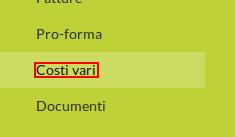
\includegraphics[width=.4\columnwidth]{images/areacliccabile.png}
	\caption{Esempio di colorazione per evidenziare la pagina corrente (l'area cliccabile è circondata dal rettangolo rosso)}
	\end{figure}
		
	\item Su \textit{\resa{}}, per chiudere la finestra del timer delle attività e necessario cliccare
	all'interno di essa. Questo presenta due problemi, il primo è che non è intuitivo dover
	cliccare su di un elemento per chiuderlo (normalmente bisogna cliccare all'esterno e questo
	è ad esempio il comportamento del menù laterale di navigazione), il secondo è che è
	possibile che un/a utente sbagli ad esempio nel cliccare il tasto "play", chiudendo la
	finestra.
	\end{itemize}
\item \textbf{Colorazione e contrasti}: tutti gli elementi di una pagina dovrebbero
essere facilmente visibili agli utenti, anche in caso di problemi di vista, ecc.
	\begin{itemize}
	\item I \textit{titoli} delle pagine, su Firefox, si vedono molto chiari sullo sfondo,
	questo potrebbe causare problemi di visualizzazione.
	
	\begin{figure}[H]\label{imgContrasti}
	\centering
	
\includegraphics[width=.4\columnwidth]{images/contrasti.png}
	\caption{Esempio di contrasto tra il titolo di una pagina e lo sfondo}
	\end{figure}
	
	\end{itemize}
\item \textbf{Coerenza e prevedibilità delle azioni degli/delle utenti}: una azione di un/a
utente dovrebbe sempre dare lo stesso risultato. Le sorprese non sono gradite e un sito
dal comportamento "imprevedibile" genera frustrazione.
	\begin{itemize}
	\item Il \textit{logo} posto in alto a sinistra sulle diverse pagine del sito dà al click
	risultati diversi in situazioni diverse: se il menù laterale è aperto, lo chiude, se invece
	il menù è chiuso, porta alla pagina di Scrivania. Questo è dovuto al fatto che
	\textit{un qualsiasi} click al di fuori del menù ne causa la chiusura, e questo evento ha
	priorità rispetto a quello di redirect sulla pagina di Scrivania. Questo però è un dettaglio
	tecnico ignoto alle/agli utenti i quali potrebbero non gradire questa diversità di esiti.
	\end{itemize}
\item \textbf{Tracciabilità del proprio percorso}: è importante per un/a utente poter
ripercorrere i propri passi all'interno di un sito web e in generale poter capire in ogni
momento a colpo d'occhio la propria posizione nella gerarchia del sito, per questo sono
utili degli strumenti come ad esempio i \textit{breadcrumb}
	\begin{itemize}
	\item Nelle pagine di secondo di livello del sito (come ad esempio la pagina di
	\textit{creazione di una nuova fattura}) non sono presenti dei breadcrumb. Per tornare alla
	pagina precedente sarebbe necessario utilizzare il tasto \textit{back} del browser oppure
	aprire il menù e riselezionarla.
	\end{itemize}
\item \textbf{Evidenziare le funzionalità}: una qualsiasi funzionalità deve sempre essere
messa chiaramente in evidenza, se un'area di testo è editabile si deve poter capire a colpo
d'occhio, se una zona è cliccabile anche, ecc.
	\begin{itemize}
	\item Su \textit{\resa{}}, nel box di creazione rapida delle attività non è immediatamente
	evidente che i valori di minuti e ore del tempo stimato siano editabili come una normale
	textbox. Gli altri campi di testo editabili sono circondati da un bordo che li identifica
	convenzionalmente come tali.
	
	\begin{figure}[H]\label{imgCreazioneAttivita}
	\centering
	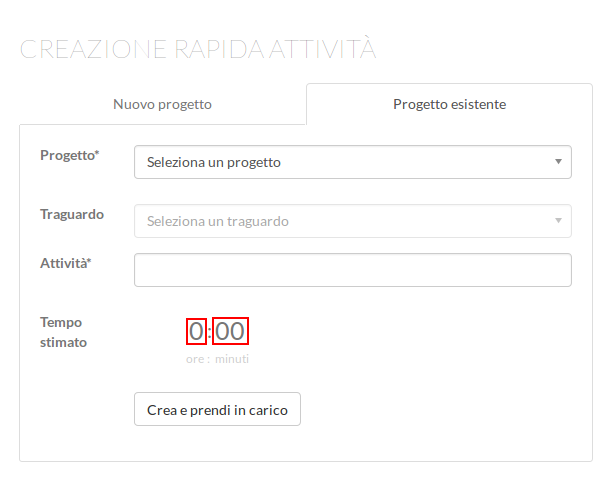
\includegraphics[width=.8\columnwidth]{images/creazioneAttivita.png}
	\caption{Box di creazione rapida delle attività, le parti circondate dai rettangoli rossi sono editabili come normali text box}
	\end{figure}
		
	\end{itemize}
\end{itemize}

\subsection{Aspetti positivi}
L'applicazione presenta alcuni aspetti positivi che contribuiscono a migliorare l'esperienza
delle/degli utenti.

\begin{itemize}
\item \textbf{Aiuto contestuale}: per un'applicazione web contemporanea non ha molto senso
fornire un manuale d'uso "classico". Gli/Le utenti sono ormai abituati/e ad esplorare da
subito le diverse funzionalità, imparando mano a mano che scoprono il prodotto.
\fiscoloWeb{} offre in diverse occasioni un aiuto contestuale, ovvero delle informazioni
semplici e rapide su come portare a termine un obiettivo, date nel contesto giusto, ovvero
quando l'utente sta effettivamente perseguendo quell'obiettivo. Oltre a questo vengono
fornite anche una guida approfondita e completa come riferimento e una funzionalità di help
che apre un box esplicativo per ogni pagina.

\begin{figure}[H]\label{imgAiutoContestuale}
\centering
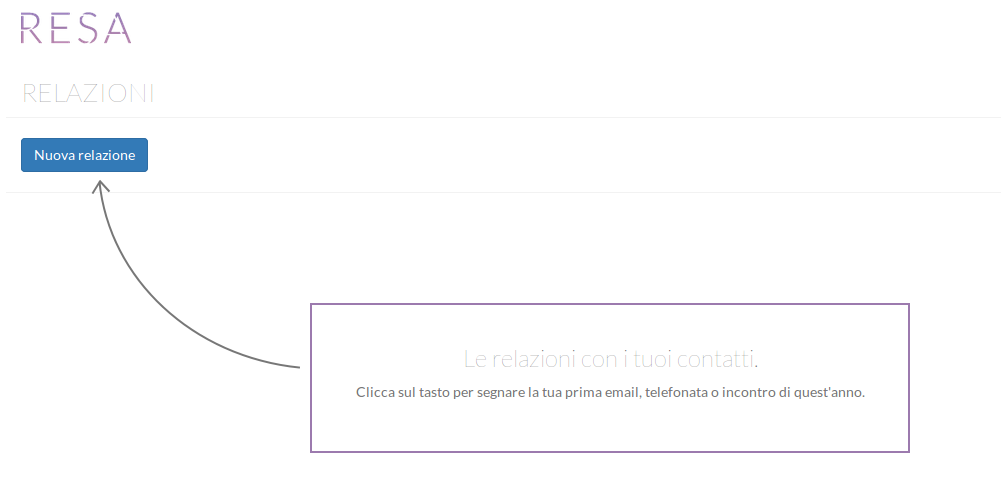
\includegraphics[width=1\columnwidth]{images/aiutoContestuale.png}
\caption{Esempio di aiuto contestuale su \resa}
\end{figure}

\item \textbf{Consistenza della presentazione grafica}: i due sottomoduli sono ben divisi
dagli schemi di colorazione e dai loghi posti in alto a sinistra delle pagine, questo permette
di capire a colpo d'occhio in che macro-area dell'applicazione ci si trova.
\end{itemize}